\chapter{Software Architecture Design}
\label{chap:software-architecture-design}
<TIP: Describe how you design your application using Unified Modelling
Language (UML). There should be at least two diagrams that describe the
software architecture. You may add additional or remove unnecessary diagrams.
However, there needs to be a coherency between them at the end./>

\section{Domain Model}
\label{section:domain-model}

\begin{figure}[h]
    \centering
    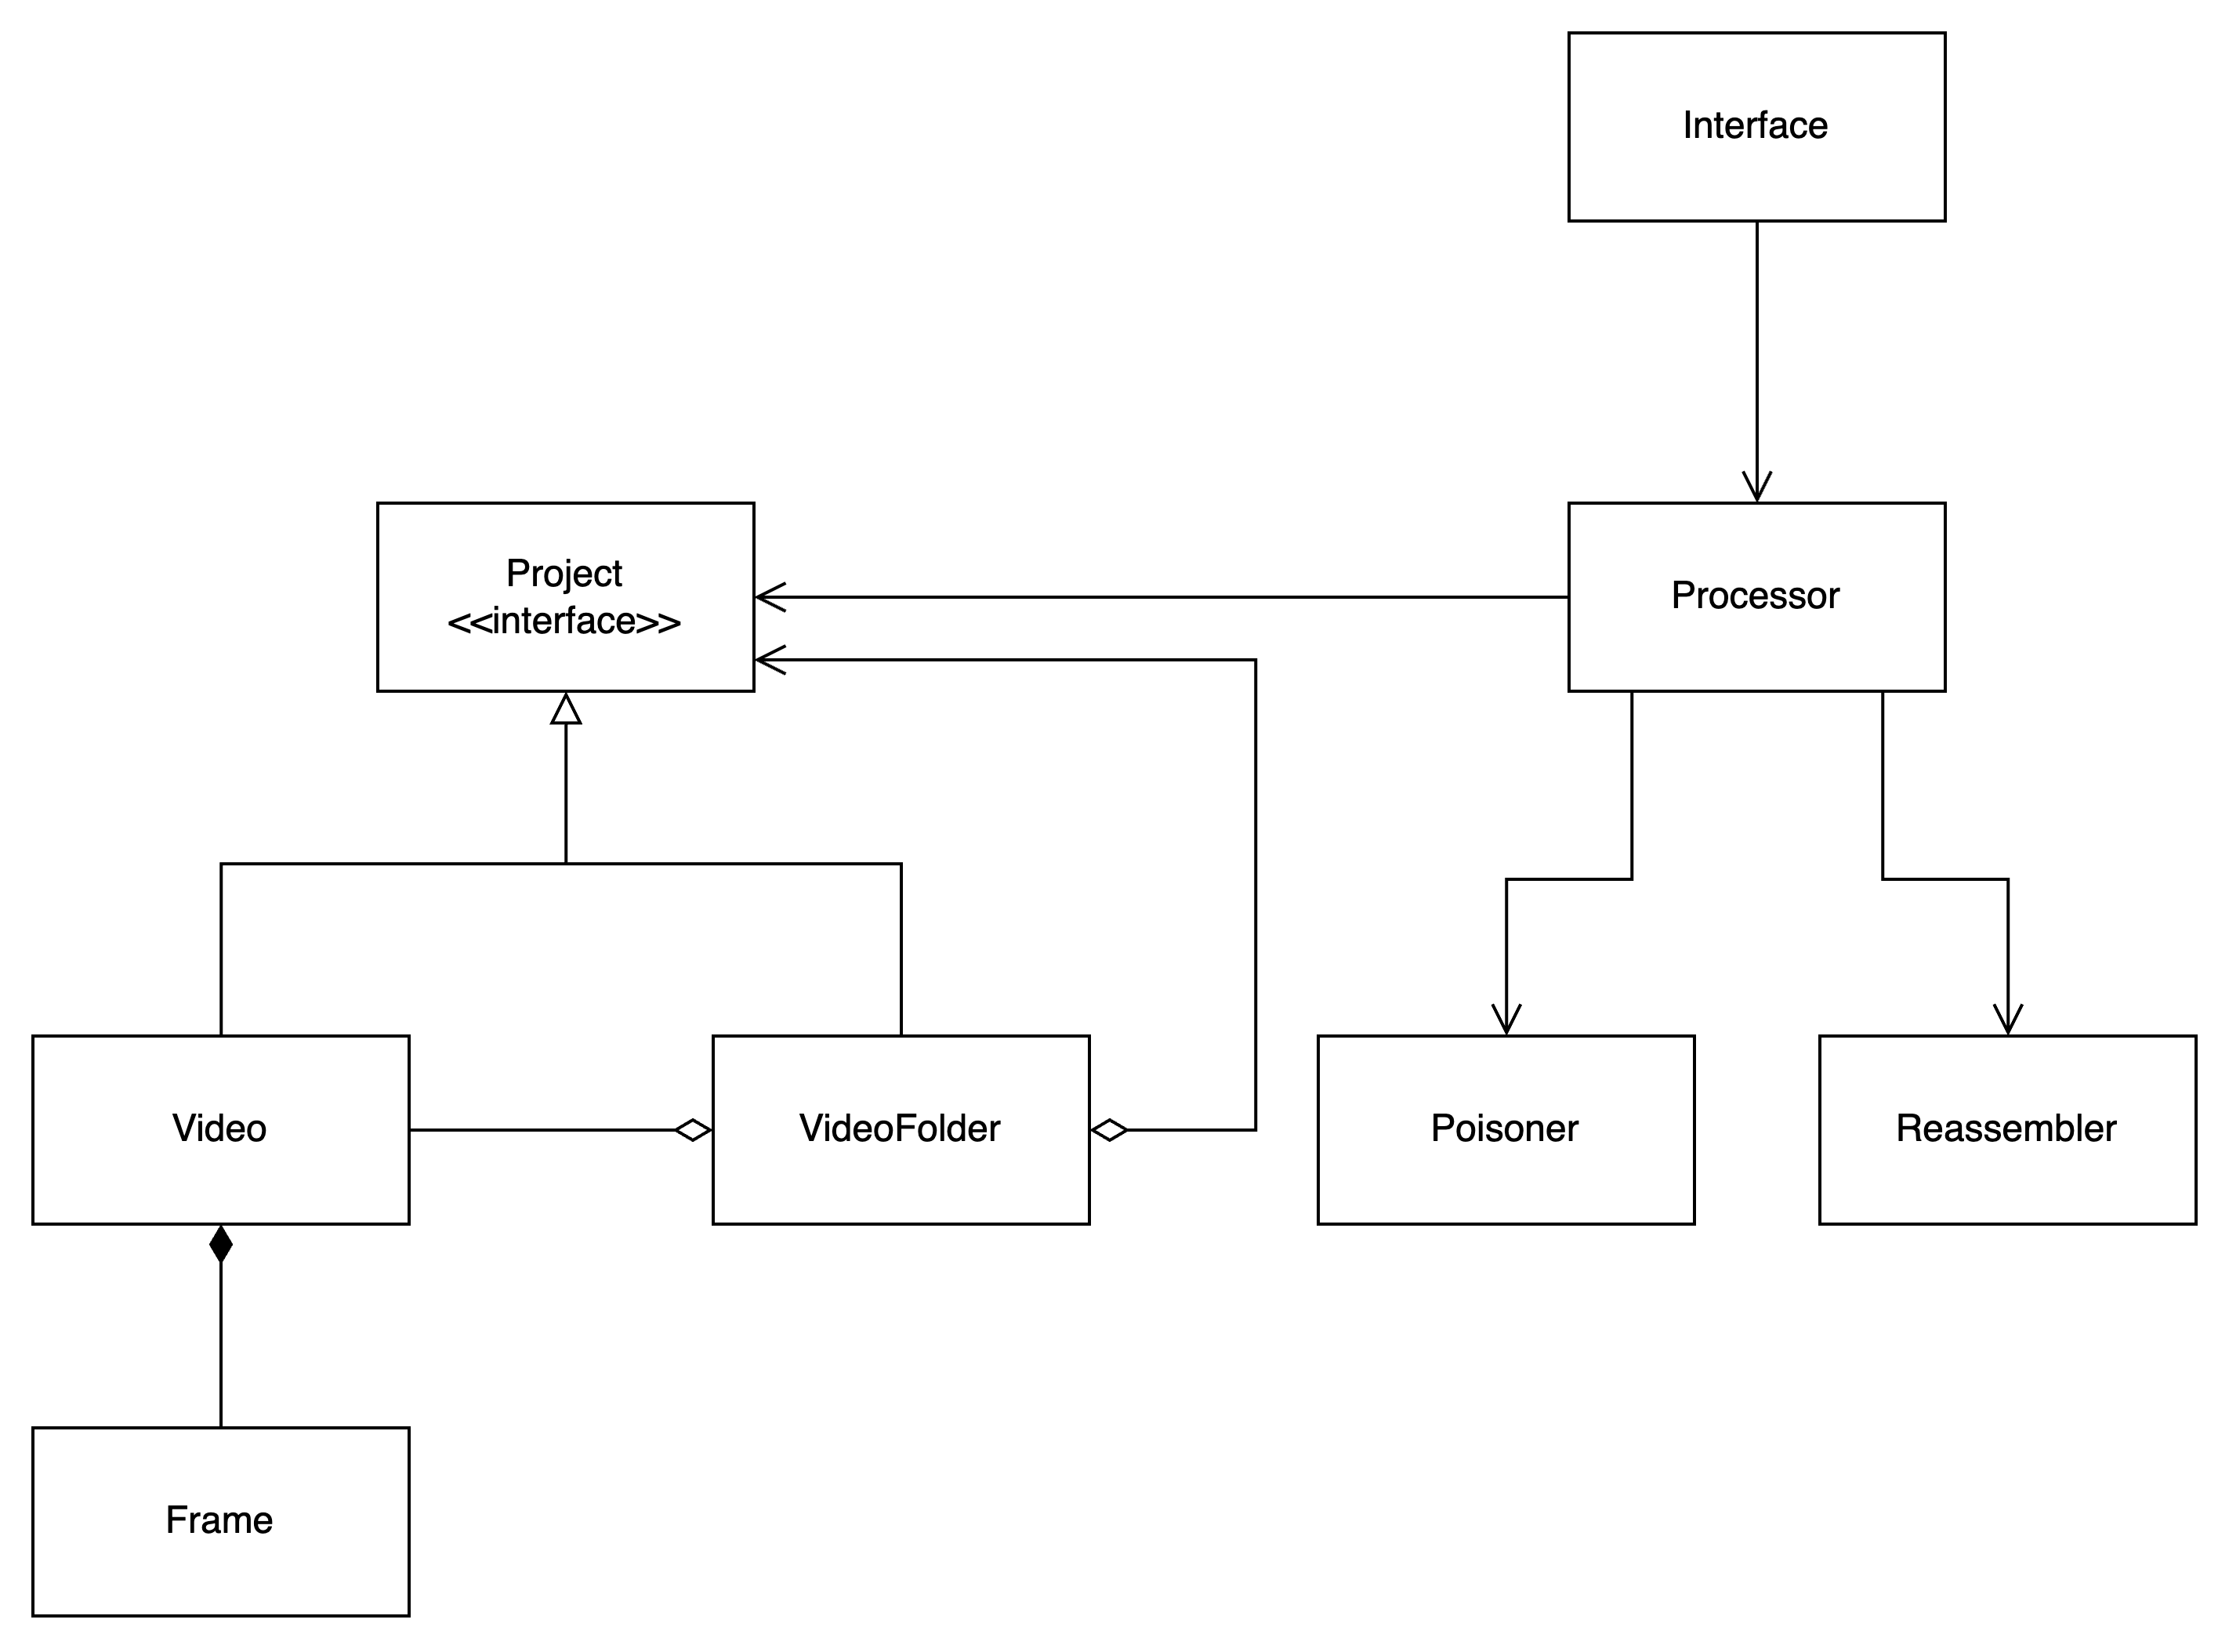
\includegraphics[width=0.8\textwidth]{chapter_4/domain model.png}
    \caption{Mockup of Main Process Design}
    \label{fig:domain-model}
\end{figure}

The domain model of Vid Scratch (Figure \ref{fig:domain-model}) represents the conceptual structure of the video poisoning system, capturing high-level components while abstracting technical complexities like file I/O or GUI rendering.

\section{Design Class Diagram}
\label{section:design-class-diagram}
<TIP: Showcase a design class diagram for your project and explain
how it works here. You can group classes into packages or layers to communicate your
design better./>

\section{Sequence Diagram}
\label{section:sequence-diagram}
<TIP: Sequence diagrams describe how the software runs at runtime.
You do not have to create a sequence diagram for every scenario. However,
there should be one for all the main ones./>

<ChatGPT: Creating a sequence diagram for every use case is not
strictly necessary, but it can be a valuable tool in certain situations. Sequence
diagrams are particularly useful for illustrating the interactions between different
components or objects in a system over time, showcasing the flow of messages
or actions between them./>

% \section{Algorithm}
% \label{section:algorithm}
% <TIP: Optional, If you are working on a research project that proposes a new
% algorithm, you can describe your algorithm here. It can be in the form of
% pseudocode or any diagram that you deem appropriate./>

\section{AI Component old}
\label{section:ai-component-old}

\subsection{Poisoning Component}
\label{subsection:poisoning-component}
\begin{enumerate}
    \item Generate Universal Adversarial Perturbation with stAdv and BTC-UAP perturbation techniques
    \item Combine Input and Generated perturbation and limit them to stay within the color value range.
    \item Ensure Output Quality with LPIPS and SSIM perceptual similarity ratings that users can set perceptual difference threshold.
    \begin{enumerate}
        \item LPIPS : ranges from 0 to infinity. High perceptual similarity is close to 0.
        \item SSIM : ranges from -1 to 1. High perceptual similarity is close to 1.
    \end{enumerate}
\end{enumerate}

\subsection{Hardware Optimization Component}
\label{subsection:hardware-optimization-component}
Before the Poisoning Process begins, perform hardware checks to minimize processing time
\begin{enumerate}
    \item detect hardware’s available CPU, GPU, SSD
    \item maximize inference distribution across available CPU / GPU by cutting Videos into smaller videos and queue through different inferences
    \item use SSD to alleviate cache from AI
    \item maximize available batch for GPU
    \item Eliminate identical frames to pick only one nearest identical frame to process through AI Pipeline with marked timestamp
\end{enumerate}
